%<dscrpt>Fichier de déclarations Latex à inclure au début d'un élément de cours.</dscrpt>

\documentclass[a4paper]{article}
\usepackage[hmargin={1.8cm,1.8cm},vmargin={2.4cm,2.4cm},headheight=13.1pt]{geometry}

%includeheadfoot,scale=1.1,centering,hoffset=-0.5cm,
\usepackage[pdftex]{graphicx,color}
\usepackage[french]{babel}
%\selectlanguage{french}
\addto\captionsfrench{
  \def\contentsname{Plan}
}
\usepackage{fancyhdr}
\usepackage{floatflt}
\usepackage{amsmath}
\usepackage{amssymb}
\usepackage{amsthm}
\usepackage{stmaryrd}
%\usepackage{ucs}
\usepackage[utf8]{inputenc}
%\usepackage[latin1]{inputenc}
\usepackage[T1]{fontenc}


\usepackage{titletoc}
%\contentsmargin{2.55em}
\dottedcontents{section}[2.5em]{}{1.8em}{1pc}
\dottedcontents{subsection}[3.5em]{}{1.2em}{1pc}
\dottedcontents{subsubsection}[5em]{}{1em}{1pc}

\usepackage[pdftex,colorlinks={true},urlcolor={blue},pdfauthor={remy Nicolai},bookmarks={true}]{hyperref}
\usepackage{makeidx}

\usepackage{multicol}
\usepackage{multirow}
\usepackage{wrapfig}
\usepackage{array}
\usepackage{subfig}


%\usepackage{tikz}
%\usetikzlibrary{calc, shapes, backgrounds}
%pour la présentation du pseudo-code
% !!!!!!!!!!!!!!      le package n'est pas présent sur le serveur sous fedora 16 !!!!!!!!!!!!!!!!!!!!!!!!
%\usepackage[french,ruled,vlined]{algorithm2e}

%pr{\'e}sentation du compteur de niveau 2 dans les listes
\makeatletter
\renewcommand{\labelenumii}{\theenumii.}
\renewcommand{\thesection}{\Roman{section}.}
\renewcommand{\thesubsection}{\arabic{subsection}.}
\renewcommand{\thesubsubsection}{\arabic{subsubsection}.}
\makeatother


%dimension des pages, en-t{\^e}te et bas de page
%\pdfpagewidth=20cm
%\pdfpageheight=14cm
%   \setlength{\oddsidemargin}{-2cm}
%   \setlength{\voffset}{-1.5cm}
%   \setlength{\textheight}{12cm}
%   \setlength{\textwidth}{25.2cm}
   \columnsep=1cm
   \columnseprule=0.5pt

%En tete et pied de page
\pagestyle{fancy}
\lhead{MPSI-\'Eléments de cours}
\rhead{\today}
%\rhead{25/11/05}
\lfoot{\tiny{Cette création est mise à disposition selon le Contrat\\ Paternité-Pas d'utilisations commerciale-Partage des Conditions Initiales à l'Identique 2.0 France\\ disponible en ligne http://creativecommons.org/licenses/by-nc-sa/2.0/fr/
} }
\rfoot{\tiny{Rémy Nicolai \jobname}}


\newcommand{\baseurl}{http://back.maquisdoc.net/data/cours\_nicolair/}
\newcommand{\urlexo}{http://back.maquisdoc.net/data/exos_nicolair/}
\newcommand{\urlcours}{https://maquisdoc-math.fra1.digitaloceanspaces.com/}

\newcommand{\N}{\mathbb{N}}
\newcommand{\Z}{\mathbb{Z}}
\newcommand{\C}{\mathbb{C}}
\newcommand{\R}{\mathbb{R}}
\newcommand{\D}{\mathbb{D}}
\newcommand{\K}{\mathbf{K}}
\newcommand{\Q}{\mathbb{Q}}
\newcommand{\F}{\mathbf{F}}
\newcommand{\U}{\mathbb{U}}
\newcommand{\p}{\mathbb{P}}


\newcommand{\card}{\mathop{\mathrm{Card}}}
\newcommand{\Id}{\mathop{\mathrm{Id}}}
\newcommand{\Ker}{\mathop{\mathrm{Ker}}}
\newcommand{\Vect}{\mathop{\mathrm{Vect}}}
\newcommand{\cotg}{\mathop{\mathrm{cotan}}}
\newcommand{\sh}{\mathop{\mathrm{sh}}}
\newcommand{\ch}{\mathop{\mathrm{ch}}}
\newcommand{\argsh}{\mathop{\mathrm{argsh}}}
\newcommand{\argch}{\mathop{\mathrm{argch}}}
\newcommand{\tr}{\mathop{\mathrm{tr}}}
\newcommand{\rg}{\mathop{\mathrm{rg}}}
\newcommand{\rang}{\mathop{\mathrm{rg}}}
\newcommand{\Mat}{\mathop{\mathrm{Mat}}}
\newcommand{\MatB}[2]{\mathop{\mathrm{Mat}}_{\mathcal{#1}}\left( #2\right) }
\newcommand{\MatBB}[3]{\mathop{\mathrm{Mat}}_{\mathcal{#1} \mathcal{#2}}\left( #3\right) }
\renewcommand{\Re}{\mathop{\mathrm{Re}}}
\renewcommand{\Im}{\mathop{\mathrm{Im}}}
\renewcommand{\th}{\mathop{\mathrm{th}}}
\newcommand{\repere}{$(O,\overrightarrow{i},\overrightarrow{j},\overrightarrow{k})$}
\newcommand{\cov}{\mathop{\mathrm{Cov}}}

\newcommand{\absolue}[1]{\left| #1 \right|}
\newcommand{\fonc}[5]{#1 : \begin{cases}#2 \rightarrow #3 \\ #4 \mapsto #5 \end{cases}}
\newcommand{\depar}[2]{\dfrac{\partial #1}{\partial #2}}
\newcommand{\norme}[1]{\left\| #1 \right\|}
\newcommand{\se}{\geq}
\newcommand{\ie}{\leq}
\newcommand{\trans}{\mathstrut^t\!}
\newcommand{\val}{\mathop{\mathrm{val}}}
\newcommand{\grad}{\mathop{\overrightarrow{\mathrm{grad}}}}

\newtheorem*{thm}{Théorème}
\newtheorem{thmn}{Théorème}
\newtheorem*{prop}{Proposition}
\newtheorem{propn}{Proposition}
\newtheorem*{pa}{Présentation axiomatique}
\newtheorem*{propdef}{Proposition - Définition}
\newtheorem*{lem}{Lemme}
\newtheorem{lemn}{Lemme}

\theoremstyle{definition}
\newtheorem*{defi}{Définition}
\newtheorem*{nota}{Notation}
\newtheorem*{exple}{Exemple}
\newtheorem*{exples}{Exemples}


\newenvironment{demo}{\renewcommand{\proofname}{Preuve}\begin{proof}}{\end{proof}}
%\renewcommand{\proofname}{Preuve} doit etre après le begin{document} pour fonctionner

\theoremstyle{remark}
\newtheorem*{rem}{Remarque}
\newtheorem*{rems}{Remarques}

\renewcommand{\indexspace}{}
\renewenvironment{theindex}
  {\section*{Index} %\addcontentsline{toc}{section}{\protect\numberline{0.}{Index}}
   \begin{multicols}{2}
    \begin{itemize}}
  {\end{itemize} \end{multicols}}


%pour annuler les commandes beamer
\renewenvironment{frame}{}{}
\newcommand{\frametitle}[1]{}
\newcommand{\framesubtitle}[1]{}

\newcommand{\debutcours}[2]{
  \chead{#1}
  \begin{center}
     \begin{huge}\textbf{#1}\end{huge}
     \begin{Large}\begin{center}Rédaction incomplète. Version #2\end{center}\end{Large}
  \end{center}
  %\section*{Plan et Index}
  %\begin{frame}  commande beamer
  \tableofcontents
  %\end{frame}   commande beamer
  \printindex
}


\makeindex
\begin{document}
\noindent

\debutcours{Séries numériques}{0.1 \tiny{ le \today}}

\section{Définitions}
\subsection{Vocabulaire}
En tant qu'objet mathématique, une série numérique est une suite de nombres réels ou complexes définie sur des entiers supérieurs ou égaux à un entier fixé $n_0$. On adopte pourtant des notations différentes:
\begin{displaymath}
  \left( \sum u_k \right)_{k\geq n_0} \text{ pour une série } \hspace{0.5cm} = \hspace{0.5cm} 
  \left( u_k \right)_{k\geq n_0} \text{ pour une suite }
\end{displaymath}
On dit aussi que $\left( \sum u_k \right)_{k\geq n_0}$ ou seulement $\sum u_k$ (s'il n'est pas utile de préciser le premier terme) est la série de terme général $u_k$.\\
La différence de vocabulaire traduit la différence de définition de la \emph{convergence} d'une suite ou d'une série. Pour définir la convergence d'une série, on introduit la \emph{suite de ses sommes partielles}: \index{sommes partielles}
\begin{displaymath}
  \left( \sum_{k=n_0}^{n}\right)n\geq n_0 .
\end{displaymath}
\begin{defi}
  Une série est convergente si et seulement si la suite de ses sommes partielles est convergente. Dans ce cas, la limite de la suite des sommes partielles est appelée la \emph{somme} de la série. Elle est notée:
  \begin{displaymath}
    \sum_{k=n_0}^{+\infty} u_k .
  \end{displaymath}
  Une série est dite divergente si et seulement si elle n'est pas convergente.
\end{defi}
\index{séries: convergence} \index{somme d'une série} \index{séries: divergence}
Pour une série \emph{convergente} (et seulement dans ce cas), on peut définir la \emph{suite de ses restes}\index{suite des restes d'une série convergente}\newline
En notant $S_n = \sum_{k=n_0}^{n} u_k$ les sommes partielles, le reste d'indice $n$ est
\begin{displaymath}
  \sum_{k=n_0}^{+\infty} u_k - S_n = \underset{m}{\lim}\left( S_m - S_{n_0}\right)
= \underset{m}{\lim}\left( \sum_{k=n+1}^m u_k\right) =  \sum_{k=n+1}^{+\infty} u_k .
\end{displaymath}
Un reste est donc encore la somme d'une série convergente. Si on note $r_n = \sum_{k=n+1}^{+\infty} u_k$ et $S$ la somme, on peut la décomposer:
\begin{displaymath}
  S = S_n + r_n .
\end{displaymath}
La suite des restes d'une série convergente converge vers $0$.
\begin{exple}
  Série de terme général $\frac{1}{k(k+1)}$.\newline
  Elle est convergente de somme $1$ car on peut obtenir une expression de la suite des sommes partielles par dominos
  \[
   \frac{1}{k(k+1)} = \frac{1}{k} - \frac{1}{k+1} \Rightarrow \sum_{k=1}^{n}\frac{1}{k(k+1)} = 1 - \frac{1}{n+1} \rightarrow 1.
  \]
\end{exple}

\begin{prop}
  Pour un entier $n_0$ donné, l'ensemble des séries convergentes définies pour les entiers plus grands que $n_0$ est un sous-espace vectoriel de l'espace des suites. La somme est une forme linéaire.
\begin{displaymath}
  \forall\lambda \in \R, \forall \left( \sum u_k \right)_{k\geq n_0}, \left( \sum v_k \right)_{k\geq n_0} \text{ convergentes }:
\left\lbrace 
\begin{aligned}
  &\left( \sum u_k + v_k\right)_{k\geq n_0}, \; \left( \sum \lambda u_k \right)_{k\geq n_0} \text{ convergentes}\\
  &\sum_{k=n_0}^{+\infty} \lambda u_k = \lambda \sum_{k=n_0}^{+\infty}  u_k\\
  &\sum_{k=n_0}^{+\infty} u_k + v_k = \sum_{k=n_0}^{+\infty} u_k + \sum_{k=n_0}^{+\infty}  v_k
\end{aligned}
\right. 
\end{displaymath}
\end{prop}
\begin{demo}
  Il suffit d'appliquer les théorèmes usuels sur les suites convergentes aux suites de sommes partielles.
\end{demo}
On pourrait avoir l'impression que les sommes partielles des séries sont des suites très particulières. En fait, n'importe quelle suite peut être considérée comme la suite des sommes partielles d'une série. Il suffit de considérer la différence entre deux termes consécutifs.\index{lien suite - série}\newline
Soit $\left( x_n\right)_{n\geq n_0}$ une suite quelconque. On peut définir une série $\left( \sum u_n\right)_{n\geq n_0}$ dont $\left( x_n\right)_{n\geq n_0}$ est la suite des sommes partielles en posant
\begin{displaymath}
\left. 
\begin{aligned}
  u_{n_0} &= x_{n_0}\\
  \forall n > n_0:\; u_{n} &= x_n - x_{n-1}  
\end{aligned}
\right\rbrace \Rightarrow
\forall n \geq n_0: \;\sum_{k=n_0}^{n}u_k = x_n
\end{displaymath}
(sommation en dominos).
\begin{defi}
  On dit que deux séries sont \emph{de même nature} si et seulement si la convergence de l'une est équivalente (logiquement) à la convergence de l'autre. Cela revient aussi à l'équivalence des divergences. 
\end{defi}


\subsection{Conditions élémentaires}
\index{divergence grossière}
\begin{prop}
  Si une série $\left( \sum u_k\right)_{k\geq n_0} $ converge, alors la suite $(u_k)_{k\geq n_0}$ converge vers $0$. Si le terme général d'une série ne converge pas vers $0$, on dit que la série est \emph{grossièrement divergente} ou \emph{trivialement divergente}.
\end{prop}
\begin{demo}
  Notons $(U_n)_{n\geq n_0}$ la suite des sommes partielles: $\forall n \geq n_0, \; U_n = \sum_{k=n_0}^{n}u_k$. Si $(U_n)_{n\geq n_0}$ converge, alors la suite extraite $(U_{n-1})_{n\geq n_0 +1}$ aussi et vers la même limite donc la différence tend vers $0$. Comme $U_n-U_{n-1}=u_n$, ceci montre que $(u_k)_{k\geq n_0}$ converge vers $0$.
\end{demo}
La convergence vers $0$ du terme général d'une série est une condition \emph{nécessaire} à la convergence de la série mais elle n'est pas \emph{suffisante}.\newline
Exemples de séries divergentes dont le terme général converge vers $0$ (non trivialement divergentes).
\begin{itemize}
 \item La série $\left( \sum \ln(1+\frac{1}{k}) \right)$ diverge bien que son terme général tende vers $0$. En effet $\ln(1+\frac{1}{k}) \sim \frac{1}{k} \rightarrow 0$ mais 
 \[
  \sum_{k=1}^{n}\ln(1+\frac{1}{k}) = \sum_{k=1}^{n}\left( \ln(1+k) - \ln(k))\right) = \ln(n+1) \rightarrow +\infty. 
 \]
 
 \item La série $\left( \sum \frac{1}{k} \right)$ dite série \emph{harmonique} \index{série harmonique} diverge bien que son terme général tende vers $0$. En effet $\frac{1}{k} \rightarrow 0$ mais
 \begin{multline*}
  \sum_{k=1}^{2^n}\frac{1}{k}\\  
  = 1 
  + \underset{> 2\times \frac{1}{4}}{\underbrace{\left( \frac{1}{2} + \frac{1}{3}\right)}} 
  + \underset{> 4 \times\frac{1}{8}}{\underbrace{\left( \frac{1}{4} + \frac{1}{5} + \frac{1}{6} +\frac{1}{7}\right)}}
  + \cdots 
  + \underset{> 2^k \times \frac{1}{2^{k+1}}}{\underbrace{\left( \frac{1}{2^{k}} + \cdots + \frac{1}{2^{k+1}-1}\right)}} + \cdots 
  + \underset{> 2^{n-1} \times \frac{1}{2^{n}}}{\underbrace{\left( \frac{1}{2^{n-1}} + \cdots + \frac{1}{2^{n}-1}\right)}}\\
  \geq 1 + \frac{n-1}{2} \rightarrow + \infty.
 \end{multline*}
\end{itemize}

\subsection{Séries géométriques}
\index{séries géométriques}
Une série géométrique de raison $q \in \C$ est convergente si et seulement si $|q|<1$. Dans ce cas, sa somme est:
\begin{displaymath}
  \sum_{n=0}^{+\infty} q^n = \frac{1}{1-q},
\end{displaymath}
sinon elle est grossièrement divergente.
\begin{demo}
Ce la résulte de l'expression des sommes partielles et de la convergence ou divergence des suites géométriques.  $(1+q+\cdots + q_n)(1-q) = 1- q^{n+1}$.
\end{demo}


\section{Séries à termes positifs}
Dans le cas particulier d'une série à termes positifs, la suite des sommes partielles est croissante. on en déduit la proposition suivante.
\begin{prop}
  Une série à termes positifs converge si et seulement si la suite de ses sommes partielles est majorée.
\end{prop}
\begin{demo}
 La suite des sommes partielles est croissante car on passe d'une somme à la suivante en ajoutant un réel positif. On en déduit qu'une suite croissante est convergente si et seulement si elle est bornée.
\end{demo}

\begin{prop}
  Soit $\left( \sum u_n\right)_{n\geq n_0}$ et $\left( \sum v_n\right)_{n\geq n_0}$ deux séries à termes positifs.
\begin{displaymath}
  \left. 
  \begin{aligned}
    &u_n \in O(v_n) \\ &\left( \sum v_n\right)_{n\geq n_0} \text{ convergente}
  \end{aligned}
  \right\rbrace 
\Rightarrow \left( \sum u_n\right)_{n\geq n_0} \text{ convergente}
\end{displaymath}
\end{prop}
\begin{demo}
Par définition de la relation de domination, il existe $K>0$ tel que $u_n \leq v_n$ pour tous les $n \geq n_0$. On en déduit que $U_n \in O(V_n)$ en notant $(U_n)$ et $(V_n)$ les suites des sommes partielles. Comme la série $\sum v_n$ converge, la suite croissante $V_n$ converge vers une limite $V$ qui est la borne supérieure de ces valeurs. D'où
\[
 \forall n \geq n_0, \; U_n \leq LV_n \leq K\, V.
\]
La suite $(V_n)$ est croissante majorée donc convergente.
\end{demo}
\begin{rem}
 Si $\sum v_n$ est convergente avec $u_n \leq v_n$ pour tous les $n$ alors $\sum u_n$ est convergente et, par passage à la limite dans une inégalité, $\sum_{k=n_0}^{+\infty} u_k \leq \sum_{k=n_0}^{+\infty} u_k$.
\end{rem}

\begin{prop}
  Si $u_n$ et $v_n$ sont les termes généraux de deux séries à termes positifs et si $u_n \sim v_n$, les séries sont de mêmes nature.
\end{prop}
\begin{demo}
  Deux suites équivalentes se dominent mutuellement. La convergence de l'une entraîne donc la convergence de l'autre. Dans ces conditions, si une des deux diverge, l'autre doit diverger également pour ne pas entrainer la convergence de la première.
\end{demo}


\section{Comparaison série - intégrale}
Le principe général est de comparer une somme partielle d'une série dont le terme général est de la forme $f(k)$ avec une intégrale de $f$ lorsque $f$ est monotone et à valeurs positives. Dans le cas où $f$ est décroissante, on peut caractériser la convergence de la série. Dans le cas où $f$ est croissante, la série est grossièrement divergente, on peut obtenir dans certains cas une équivalence pour la suite des sommes partielles.

\begin{figure}[ht]
    \centering
    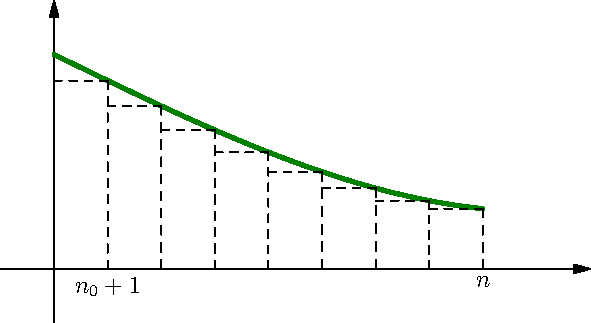
\includegraphics[width=7cm]{./C9650_1.pdf}
    \caption{$\sum_{k=n_0}^{n}f(k) \leq f(n_0) +\int_{n_0}^nf(t)\,dt$}
    \label{fig:C9650_1}
\end{figure}

\begin{figure}[ht]
    \centering
    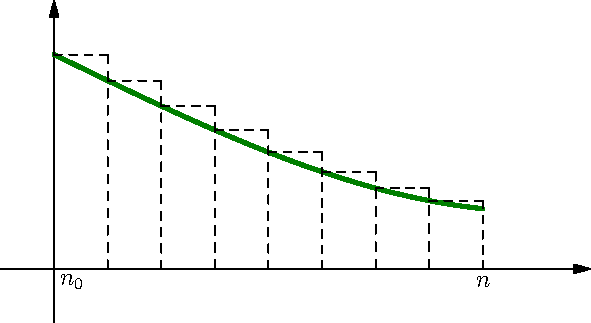
\includegraphics[width=7cm]{./C9650_2.pdf}
    \caption{$\int_{n_0}^nf(t)\,dt \leq \sum_{k=n_0}^{n-1}f(k)$}
    \label{fig:C9650_2}
\end{figure}

\begin{prop}
  Soit $f$ une fonction continue dans un intervalle $[n_0,+\infty[$ et à valeurs positives. Pour $k\geq n_0$, on note $u_k=f(k)$.
\begin{itemize}
  \item Si $f$ est décroissante, la série $\left( \sum u_k \right)_{k\geq n_0}$ est convergente si et seulement si les primitives de $f$ ont une limite finie en $+\infty$.
  \item Si $f$ est croissante, la série $\left( \sum u_k \right)_{k\geq n_0}$ est grossièrement divergente.
\end{itemize}
\end{prop}
\begin{demo}
Comme la fonction est à valeurs positives, la suite des sommes partielles est croissante, les primitives sont croissantes. Les convergences sont donc équivalentes au caractère borné de la suite ou d'une primitive. On forme des inégalités à l'aide des figures 1 à 4 dans lesquelles l'aire de chaque rectangle en pointillé est un terme de la série puisque sa largeur est 1.\newline
Dans le cas où la fonction est décroissante.\newline
Si les primitives convergent en $+\infty$, la majoration des sommes partielles qui se déduit de la figure \ref{fig:C9650_1} montre la convergence de la série. Si la série converge, la figure \ref{fig:C9650_2} permet de majorer une primitive et de prouver sa convergence.\newline
Si la fonction est croissante, la suite des $f(k)$ ne converge pas vers $0$ car tous ses termes sont plus grands que $f(n_0)$, la série est trivialement divergente. Notons $F$ la primitive nulle en $n_0$ et $S_n$ une somme partielle.
\begin{displaymath}
 S_n = \sum_{k=n_0}^{n}f(k),\hspace{1cm} F(t) \geq (t-n_0)f(n_0) \Rightarrow f \xrightarrow{+\infty} +\infty
\end{displaymath}
\end{demo}
Dans le cas où la fonction croissante, on peut montrer (sous une hypothèse supplémentaire) que la suite des sommes partielles $\sum_{k=n_0}^n u_k$ est équivalente à la suite des $F(n)$. Les figures \ref{fig:C9650_3} et \ref{fig:C9650_4} conduisent à l'encadrement suivant:
\begin{displaymath}
F(n) + f(n_0) \leq S_n \leq F(n) +f(n) \Rightarrow 1 + \frac{f(n_0)}{F(n)} \leq \frac{S_n}{F(n)} \leq 1 + \frac{f(n)}{F(n)}
\end{displaymath}
La figure \ref{fig:C9650_3} pour l'inégalité à gauche et \ref{fig:C9650_4} pour l'inégalité à droite. Comme $F$ diverge vers $+\infty$ en $+\infty$ et que $f(n_0)$ est fixé, les deux suites sont équivalentes si et seulement si $f(n)$ est négligeable devant $F(n)$.\newline
Ce n'est pas toujours réalisé, par exemple pour la fonction exponentielle.
\begin{figure}[ht]
    \centering
    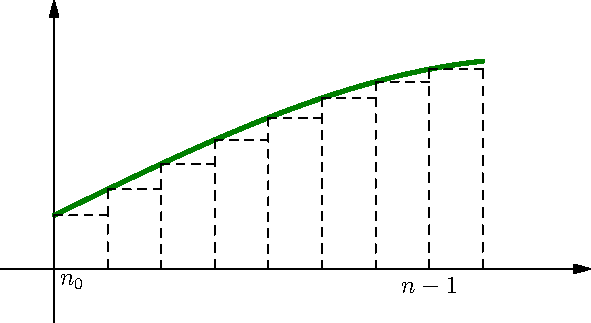
\includegraphics[width=7cm]{./C9650_3.pdf}
    \caption{$\sum_{k=n_0}^{n-1}f(k) \leq \int_{n_0}^nf(t)\,dt$}
    \label{fig:C9650_3}
\end{figure}
\begin{figure}[ht]
    \centering
    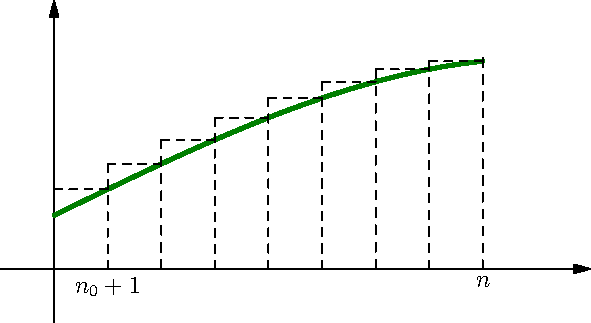
\includegraphics[width=7cm]{./C9650_4.pdf}
    \caption{$\int_{n_0}^nf(t)\,dt \leq -f(n_0)+\sum_{k=n_0}^{n}f(k)$}
    \label{fig:C9650_4}
\end{figure}

Appliquons la propriété précédente à deux séries usuelles.
\begin{prop}
$\alpha$ et $\beta$ sont des réels:
\begin{itemize}
  \item Série de Riemann \index{série de Riemann}: de terme général $\frac{1}{n^\alpha}$. Elle converge si et seulement si $\alpha >1$.
  \item Série de Bertrand \index{série de Bertrand}: de terme général $\frac{1}{n^\alpha(\ln n)^\beta}$. Elle converge si et seulement si $\alpha >1$ ou $\alpha = 1$ et $\beta>1$.
\end{itemize}  
\end{prop}
\begin{demo}
  Rappelons des primitives connues:
\begin{center}
\renewcommand{\arraystretch}{1.6}
\begin{tabular}{|l|l|} \hline
fonction & primitive \\ \hline
$\frac{1}{t^\alpha}$ & $-\frac{1}{\alpha -1}\frac{1}{t^{\alpha -1}}$ \\ \hline
$\frac{1}{t\ln t}$ & $\ln(\ln t)$ \\\hline
\end{tabular}
\end{center}
Les séries considérées sont à termes positifs à partir d'un certain rang. Pour $\alpha$ et $\beta$ positifs, les fonctions associées sont positives et décroissantes.
\end{demo}


\section{Séries absolument convergentes}
\index{série absolument convergente}
\begin{defi}
  Une série est dite \emph{absolument} convergente si et seulement si la série de ses valeurs absolues (ou modules dans le cas complexe) est convergente.
\end{defi}
\begin{prop}
  Une série absolument convergente est convergente. Le module de la somme est alors inférieur ou égal à la somme des modules.
\end{prop}
\begin{demo}
Considérons une série à valeurs complexes $\left( \sum z_n\right)_{n \in \N}$ et la série des modules $\left( \sum |z_n|\right)_{n \in \N}$ qui est supposée convergente. Les sommes partielles sont notées
\[
 Z_n = \sum_{k=0}^n z_k\; \text{ et } T_n = \sum_{k=0}^n |z_k|.
\]
Décomposons $z_n$ en parties réelle et imaginaire puis chacun de ces nombres réels en parties positives et négatives. Rappelons les définitions et propriétés:
\[
 \forall x \in \R,\; x_+ = \max(x,0)\geq 0, \, x_- = \max(-x,0) \geq 0,\, x = x_+ - x_-,\, |x| = x_+ + x_-.  
\]
Introduisons des notations:
\[
\left. 
\begin{aligned}
 a_n &= \Re(z_n)_+ &, A_n &= \sum_{k=0}^n a_k ; & &
 b_n &= \Re(z_n)_- &, B_n &= \sum_{k=0}^n b_k \\
 c_n &= \Im(z_n)_+ &, C_n &= \sum_{k=0}^n c_k ; & &
 d_n &= \Im(z_n)_+ &, D_n &= \sum_{k=0}^n d_k 
\end{aligned}
\right\rbrace \Rightarrow 
\left\lbrace 
\begin{aligned}
z_n &= a_n - b_n + ic_n -id_n \\
Z_n &= A_n - B_n + iC_n -iD_n
\end{aligned}
\right. .
\]
La série à termes positifs $\left( \sum a_n\right)_{n \in \N}$ est convergente car 
\[
 a_n \leq |a_n| \leq |z_n| .
\]
La suite des $A_n$ est donc convergente et il en est de même pour $B_n$, $C_n$ et $D_n$. Par linéarité, on en déduit la convergence de $Z_n$.\newline
De plus
\[
 \left( \forall n \in \N, \; \left| \sum_{k=0}^{n} z_k \right| \leq \sum_{k=0}^{n} |z_k|\right)  
 \Rightarrow 
 \left| \sum_{k=0}^{+\infty} z_k \right| \leq \sum_{k=0}^{+\infty} |z_k|
\]
par passage à la limite dans une inégalité.
\end{demo}
\index{série semi-convergente}
Exemple série de Riemann complexe. Soit $\alpha\in \C$, la série de terme général $n^{-\alpha}$ est absolument convergente pour $\Re(\alpha)>1$. La somme de la série est la très célèbre fonction $\zeta$ de Rieman \index{fonction $\zeta$ de Riemann}.
\begin{defi}
  Une série convergente mais non absolument convergente est dite \emph{semi-convergente}
\end{defi}
\begin{exple}
La série harmonique alternée est semi-convergente.\index{série harmonique alternée}
à compléter 
\end{exple}

\begin{prop}
  Soit $\left( u_n\right)_{n\geq n_0}$ une suite complexe, $\left( v_n\right)_{n\geq n_0}$ une suite de réels positifs:
\begin{displaymath}
\left. 
\begin{aligned}
  &\left( u_n\right)_{n\geq n_0} \in O\left(\left( v_n\right)_{n\geq n_0} \right) \\
  & \left(\sum v_n\right)_{n\geq n_0} \text{ converge}
\end{aligned}
\right\rbrace \Rightarrow
\left( \sum u_n\right)_{n\geq n_0} \text{ absolument convergente}
\end{displaymath}
\end{prop}
\begin{demo}
  à compléter
\end{demo}

\section{Représentation décimale des réels}
\begin{defi}\index{nombre décimal}
  Pour tout $n\in \N$, on note $\D_n = 10^{-n}\,\Z$ l'ensemble des multiples de $10^{-n}$ et $\D = \bigcup_{n\in \N}\Z \times 10^{-n}$. Un nombre décimal est un élément de $\D$.
\end{defi}
Autrement dit, un réel $x$ est un décimal si et seulement si il existe $n\in \N$ tel que $x$ soit un multiple de $10^{-n}$ c'est à dire si et seulement si $10^{n}x$ est entier. On peut remarquer que tout nombre décimal est rationnel ($\D \subset \Q$).\newline
\index{approximation décimale par défaut} 
\begin{propn} \label{appdec}
Pour tout $n\in \N$ et $x$ réel, il existe un unique $a_n(x)\in \D_n$ tel que $a_n(x)\leq x < a_n(x) + 10^{-n}$.\newline
Ce nombre $a_n(x)$ est l'\emph{approximation décimale par défaut à l'ordre $n$} de $s$. Il vérifie
\[
 a_n(x) = \frac{\lfloor10^n\, x\rfloor }{10^n}.
\]
\end{propn}
\begin{demo}
 Analyse. 
\[
 a_n(x)\leq x < a_n(x) + 10^{-n} \Rightarrow \underset{\in \Z}{\underbrace{10^n\,a_n(x)}}\leq 10^n\,x < a_n(x)x + 1
 \Rightarrow 10^n\,a_n(x) = \lfloor 10^n\,x \rfloor \Rightarrow a_n(x) = \frac{\lfloor 10^n\,x \rfloor}{10^n}.
\]
Ceci assure l'unicité.\newline
Synthèse. Le $a_n(x) = \frac{\lfloor 10^n\,x \rfloor}{10^n}$ vérifie la condition requise d'après les propriétés de la fonction partie entière. 
\end{demo}
\begin{rems}
 Avec la définition et le théorème d'encadrement, il est évident que la suite $\left( a_n(x) \right)_{n \in \N} \rightarrow x$.\newline
 On peut aussi remarquer que $a_0(x) = \lfloor x \rfloor$.\newline
 Dans le cas particulier où $x$ est décimal, la suite $a_n(x)$ est stationnaire. Pour $n$ assez grand, elle est constante de valeur $x$
\end{rems}

\begin{nota}
 On note $m_n(x) = \lfloor 10^n\, x\rfloor \in \Z$ et $r_n(x) = x - a_n(x) \in \left[ 0, 10^{-n}\right[$ de sorte que 
\[
 a_n(x) = \frac{m_n(x)}{10^n}, \hspace{0.5cm} x = \underset{\in \D_n}{\underbrace{a_n(x)}} + \underset{\in \left[ 0, 10^{-n}\right[ }{\underbrace{r_n(x)}}.
\]
Pour tout $n\in \N$, on définit aussi $d_{n+1}(x) = \lfloor 10^{n+1}\,r_n(x) \rfloor$. 
Par définition, $d_n(x) \in \llbracket 0, 9\rrbracket$ (entier entre 0 et 9) car 
\[
 r_n(x) \in \left[ 0, 10^{-n}\right[ \Rightarrow 10^{n+1}r_n(x) \in \left[ 0, 10\right[
 \Rightarrow \lfloor 10^{n+1}\,r_n(x) \rfloor  \in \llbracket 0, 9\rrbracket.
\]
\end{nota}
\begin{rems}
 La série $\left( \sum \frac{d_k(x)}{10^k} \right)_{n \in \N^*}$ est convergente car elle est à termes positifs et majorée par la série géométrique convergente $9\left( \sum \frac{1}{10^k} \right)_{n \in \N^*}$.\newline
 Si $x$ est décimal, les $r_n()$ et les $d_n(x)$ sont nuls à partir d'un certain rang.
\end{rems}

\begin{propn} \label{devdec}
 Pour $x$ réel et $n\in \N$, avec les notations précédentes:
\[
 m_{n+1}(x) = 10\,m_n(x) + d_{n+1}(x),\hspace{0.5cm}
 a_n(x) = a_0(x) + \frac{d_1(x)}{10} + \frac{d_2(x)}{10^2} + \cdots + \frac{d_n(x)}{10^n},\hspace{0.5cm}
 r_n(x) = \sum_{k = n+1}^{+\infty} \frac{d_k(x)}{10^k}.
\]
\end{propn}
\begin{demo}
En utilisant la notation $\{ \}$ pour le reste de la partie entière qui est un élément de $\left[ 0,1\right[$ :
\[
 10^{n+1}\, r_n(x) = d_{n+1}(x) + \left\lbrace 10^{n+1}\, r_n\right\rbrace 
 \Rightarrow 
 x = a_n(x) + r_n(x) 
 = \underset{ \in \D_{n+1}}{\underbrace{a_n(x) + \frac{d_{n+1}(x)}{10^{n+1}}}} 
 + \underset{\in \left[ 0,\frac{1}{10^{n+1}}\right[ }{\underbrace{\frac{\left\lbrace 10^{n+1}\, r_n\right\rbrace}{10^{n+1}}}}. 
\]
Cette relation caractérise l'unique approximation décimale de $x$ à l'ordre $n+1$:
\[
 a_{n+1}(x) = a_n(x) + \frac{d_{n+1}(x)}{10^{n+1}}
 \Rightarrow
 m_{n+1}(x) = 10^{n+1}a_{n+1}(x) = 10\, m_n(x) + d_n(x).
\]
Le développement décimal de l'approximation:
\[
 a_n(x) = a_0(x) + \frac{d_1(x)}{10} + \frac{d_2(x)}{10^2} + \cdots + \frac{d_n(x)}{10^n}
\]
se déduit immédiatement par récurrence de la relation $a_{n+1}(x) = a_n(x) + \frac{d_{n+1}(x)}{10^{n+1}}$.\newline
On a déjà signalé la convergence de la série des $\frac{d_k(x)}{10^{k}}$. On peut donc considérer librement la somme et les restes de cette série. Considérons des entiers $n$ et $p$ avec $n < p$. Alors:
\[
 \sum_{k=n+1}^{p}\frac{d_k(x)}{10^{k}} = a_p(x) - a_n(x)
 \Rightarrow
 \sum_{k=n+1}^{+ \infty}\frac{d_k(x)}{10^{k}} = x - a_n(x) = r_n(x)
\]
en passant à la limite dans les suites en $p$.
\end{demo}
\index{représentation décimale des réels}
\begin{defi}
La suite $d(x) = \left( d_n(x)\right)_{n\in \N^*}$ est la suite des décimales de $x$ \index{développement décimal} de $x$. Elle donne le \emph{développement décimal propre} de $x$ c'est à dire son écriture comme la somme d'une série
\[
 x = \lfloor x \rfloor + \sum_{k=1}^{+\infty} \frac{d_k(x)}{10^k} \hspace{0.5cm} \text{avec } \mu \in \Z \text{ et } d_k(x) \in \llbracket 0,9 \rrbracket.
\] 
\end{defi}

\begin{propn}
 Si $x$ n'est pas décimal, l'expression de $x$ comme une série de la forme précédente est unique. C'est à dire que si
\[
 x = \mu + \sum_{k=1}^{+\infty} \frac{\delta_k}{10^k} \hspace{0.5cm} \text{avec } \delta_k \in \llbracket 0,9 \rrbracket.
\]
alors $\mu = \lfloor x \rfloor$ et $\delta_k = d_k(x)$ pour tous les $k \in \N^*$.
\end{propn}
\begin{demo}
Un point essentiel est que 
\[
\sum_{k=n+1}^{+\infty}\frac{1}{10^k} = \frac{1}{10^{n+1}}\,\frac{1}{1-\frac{1}{10}} = \frac{1}{9\times 10^n}.
\]
On en déduit que, pour tout $n$,
\[
 x = \underset{ \in \D_n}{\underbrace{\mu + \sum_{k=0}^{n}\frac{\delta_k}{10^k}}} 
 + \underset{ \in \left[ 0,\frac{1}{10^{n}}\right] }{\underbrace{\sum_{k=n+1}^{+\infty}\frac{\delta_k}{10^k}}}\; \text{ car } \delta_k \in \llbracket 0,9\rrbracket.
\]
Comme $x$ \emph{n'est pas décimal}, aucun des restes $\sum_{k=n+1}^{+\infty}\frac{\delta_k}{10^k}$ ne peut être égal à $\frac{1}{10^n}$. L'écriture précédente est donc l'unique approximation décimale de $x$ à l'ordre $n$. Ceci assure l'unicité.
\end{demo}
\begin{rem}
 Si $x$ est décimal, il s'exprime de plusieurs manières comme la somme d'une série de ce type. Par exemple pour $x=1$,
\[
 1 = 1 + \sum_{k=1}^{+\infty} \frac{0}{10^{k}} \;\text{ (développement propre) et } \; 1 = 0 + \sum_{k=1}^{+\infty} \frac{9}{10^{k}}.
\]
car $\sum_{k=1}^{+\infty} \frac{1}{10^{k}} = \frac{1}{10}\,\frac{1}{1 - \frac{1}{10}} = \frac{1}{9}$
\end{rem}
Les propositions suivantes caractérisent les nombres rationnels mais elles ne figurent pas dans le programme de la classe.
\begin{propn}
 Avec les notations précédentes. Si la suite des décimales $\left( d_n(x) \right)_{n \in \N^*}$ est périodique à partir d'un certain rang alors $x$ est rationnel. 
\end{propn}
\begin{demo}
 On suppose $\left( d_n(x) \right)_{n \geq 1}$ périodique de période $l$ à parir d'un rang $s$. Notons
\[
 y = \frac{d_{s+1}(x)}{10^{s+1}} + \frac{d_{s+2}(x)}{10^{s+2}} + \cdots + \frac{d_{s+l}(x)}{10^{s+l}}.  
\]
Utilisons l'expression du reste de l'approximation comme reste d'une série (prop \ref{devdec}):
\[
 r_{s}(x) = \sum_{k=s+1}^{+\infty}\frac{d_k(x)}{10^k}
 = y + \sum_{k=s+1+l}^{+\infty}\frac{d_k(x)}{10^k}
 = y + \sum_{k'= s+1}^{+\infty}\frac{d_{k'+l}(x)}{10^{k'+l}}
\]
avec le changement d'indice $k' = k - l$ dans le reste de la série. En factorisant $10^{l}$ et avec la périodicité:
\[
 r_s(x) = y + \frac{1}{10^l}r_s(x) \Rightarrow r_s(x) = \frac{10^l\,y}{10^l - 1} \in \Q.
\]
On en déduit que $x$ est rationnel. 
\end{demo}
\begin{propn}
 Avec les notations précédentes. Si $x$ est rationnel, la suite $\left( d_n(x) \right)_{n \in \N^*}$ de ses décimales est périodique à partir d'un certain rang. 
\end{propn}
\begin{demo}
 On suppose $x$ rationnel égal à $\frac{p}{q}$ avec $p\in \Z$ et $q\in \N^*$.\newline
 Pour tout $n$, notons $\rho_n$ le reste de la division de $10^n\,p$ par $q$ et considérons la suite des $\rho_n$.\newline
 Comme elle est à valeurs dans l'ensemble fini $\llbracket 1, q-1\rrbracket$, elle ne peut être injective. Il existe donc des naturels non nuls $s$ et $s$ tel que 
 \[
  \rho_{s + l} = \rho_s .
 \]
Montrons par récurrence que la suite des $\rho$ est $l$-périodique à partir de $s$. La récurrence est initialisée par la définition de $s$ et $l$. Si $\rho_{k + l} = \rho_k$ pour un $k \geq s$, considérons les congruences modulo $q$:
\[
 \rho_{k + 1 + l} \equiv 10^{k+1+l}\, p \equiv 10\, \times \underset{ \equiv \rho_{k + l} \equiv \rho_k}{\underbrace{10^{k+l}\, p}} 
 \equiv  10\times \rho_{k} \equiv 10\times 10^k\, p \equiv \rho_{k+1}
 \Rightarrow \rho_{k + 1 + l} = \rho_{k + 1}.
\]
D'autre part, la suite des $\rho_n$ est liée à celle des restes décimaux. \'Ecrivons les divisions euclidiennes
\[
 10^n\,p = q \theta_n + \rho_n
 \Rightarrow
 x = \frac{p}{q} = \underset{\in \D_n}{\underbrace{\frac{\theta_n}{10^n}}} + \frac{\rho_n}{10^n\, q}\; \text{ avec }
 \frac{\rho_n}{10^n\, q} \in \left[ 0, \frac{1}{10^n}\right[ \text{ car } 0 \leq \rho_n < q .
\]
C'est l'unique écriture de l'approximation décimale de $x$ à l'ordre $n$ donc
\[
 r_n(x) = \frac{\rho_n}{10^n\, q}
 \Rightarrow d_{n+1}(x) = \lfloor 10^{n+1}\,r_n(x) \rfloor = \lfloor \frac{10\, \rho_n}{q}\rfloor.
\]
La périodicité de la suite des $\rho_n$ entraine celle des $d_n(x)$.
\end{demo}

\end{document}
